\documentclass[12pt]{article}
\usepackage[margin=1in]{geometry}
\usepackage{times}
\usepackage{booktabs}
\usepackage[hidelinks]{hyperref}
\usepackage{array}
\usepackage{tabularx}
\usepackage{enumitem}
\usepackage{setspace}
\usepackage{parskip}
\usepackage{graphicx}
\usepackage{caption}
\usepackage{multirow}
\usepackage{tikz}
\usetikzlibrary{shapes,arrows,positioning,calc}

\setlength{\parindent}{0pt}
\setlength{\parskip}{6pt}
\onehalfspacing

\begin{document}

\begin{center}
\textbf{Submission for Extended Experimental Scope}\\[0.5em]
\textbf{Focusing on Cross-Domain / Cross-Population Evaluation}\\[1em]
\textbf{Course: 04990-ResearchProject}\\
\textbf{Name: Moise Iradukunda Ingabire}\\
\textbf{AndrewId: mii}
\end{center}

\bigskip

%==========================================================================
\section*{I.\quad Foundation \& Extension Rationale}

\subsection*{A.\quad Baseline Achievements (Compliance Auditor v1.0)}

The initial compliance auditor system successfully demonstrated AI-augmented compliance auditing for Rwanda's NCSA Minimum Cybersecurity Standards, achieving:

\begin{itemize}
    \item 99.99\% F1-score ($\pm$0.01\%) on synthetic training data (5-fold cross-validation, $n=200,000$)
    \item 99.88\% F1-score on real SecRepo SSH authentication logs after 5\% fine-tuning (2,170 samples)
    \item \textbf{100\% zero-shot accuracy} with MCP+LLM semantic analysis on the same authentication logs
    \item 143 NCSA controls implemented (85\% coverage), with 60 specialized evidence parsers
    \item Rapid convergence: XGBoost inference at 0.32ms (p50), 5.40ms (p95)
    \item Validated hybrid fitness combining rule-based fast path (60--70\% of logs, $<$1ms) and LLM semantic path (30--40\% of logs, 280ms)
\end{itemize}

\subsection*{B.\quad Research Gap \& Extension Objective}

\textbf{Limitation:} The cross-dataset evaluation was confined to a single log type (SecRepo SSH authentication logs) and a single regulatory framework (Rwanda NCSA). The 100\% zero-shot accuracy claim is therefore specific to authentication event semantics and NCSA control semantics---not a validated general claim.

\textbf{Extension Goal:} Demonstrate that the validated MCP+LLM semantic analyzer generalizes across:

\begin{enumerate}
    \item \textbf{Multiple log types:} Authentication, firewall/network, Windows Security Events, application/API logs, and cloud audit trails
    \item \textbf{Multiple African regulatory frameworks:} Rwanda NCSA, Kenya Computer Misuse \& Cybercrimes Act 2024, Nigeria NITDA Cybersecurity Framework, South Africa POPIA/PAIA-aligned controls
    \item \textbf{Multiple deployment environments:} Cloud API (Claude/GPT-4), on-premise quantized LLMs (Llama-3.1-8B, Mistral-7B), and hybrid routing
\end{enumerate}

\textbf{Hypothesis:} A prompt-adaptive MCP+LLM architecture, combined with a cross-framework control mapping database and multi-source log normalization pipeline, enables semantic compliance analysis that generalizes across structurally distinct log formats and overlapping African regulatory frameworks without retraining the underlying classification model.

\bigskip

%==========================================================================
\section*{II.\quad Proposed Dataset: Multi-Log-Type, Multi-Framework Corpus}

\subsection*{A.\quad Data Sources}

\begin{table}[h]
\centering
\caption{Proposed Cross-Domain Dataset Composition}
\label{tab:dataset}
\begin{tabular}{@{}p{3.5cm}p{2.5cm}p{2cm}p{2cm}p{3cm}@{}}
\toprule
\textbf{Source} & \textbf{Category} & \textbf{Log Type} & \textbf{Count} & \textbf{Regulatory Coverage} \\
\midrule
SecRepo auth.log~[1] & Authentication & SSH / PAM & 86,839 & NCSA AC-7, IA-2 (baseline) \\
LogHub BGL~[2] & System & Linux kernel & 50,000 & NCSA AU-2, CM-6 \\
LogHub HDFS~[2] & Distributed sys. & Hadoop & 50,000 & NCSA SC-28, AU-9 \\
EVTX-ATTACK-SAMPLES~[3] & Windows Events & WinEvt & 30,000 & NCSA AC-2, IA-5, SI-4 \\
CICIDS 2017~[4] & Network/Firewall & PCAP/flows & 40,000 & NCSA SC-7, SI-3 \\
Kenya Synthetic & API / Audit logs & JSON/CEF & 20,000 & Kenya CMCA 2024 \\
Nigeria Synthetic & System events & Syslog & 20,000 & NITDA Cybersec. Framework \\
South Africa Synth. & Application logs & Apache/Nginx & 15,000 & POPIA data protection \\
\midrule
\textbf{Total} & \multicolumn{2}{c}{\textbf{8 sources, 5 log types}} & \textbf{311,839} & \textbf{4 regulatory frameworks} \\
\bottomrule
\end{tabular}
\end{table}

\subsection*{B.\quad Selection Criteria}

\begin{itemize}
    \item Publicly available or synthetically reproducible (no production PII)
    \item Covers at least one NCSA control family per source
    \item Structural diversity: timestamp formats, severity schemas, field names must differ across sources
    \item Minimum 15,000 events per source to support statistically valid cross-domain evaluation
    \item Synthetic African-framework logs: generated using realistic event templates derived from the published regulatory frameworks~[5,6,7]
\end{itemize}

\textbf{Exclusion Criteria:}
\begin{itemize}
    \item Logs requiring proprietary decryption or tool chains
    \item Sources with known label contamination (e.g., KDD Cup 99 without NSL correction)
    \item Sources with $>$90\% structural overlap with existing training data (SecRepo auth.log)
\end{itemize}

\subsection*{C.\quad Log Type Categorization Schema}

\begin{table}[h]
\centering
\caption{Log Type Categorization and NCSA Control Family Coverage}
\label{tab:log_types}
\begin{tabular}{@{}p{3cm}p{3cm}p{4cm}p{3cm}@{}}
\toprule
\textbf{Log Category} & \textbf{Format} & \textbf{Example Events} & \textbf{NCSA Families} \\
\midrule
Authentication & Syslog / PAM & Failed SSH, MFA bypass, account lockout & AC, IA \\
System / Kernel & Syslog / BGL & Kernel panics, process spawns, service stops & AU, CM \\
Network / Firewall & NetFlow / PCAP & Port scans, blocked connections, DDoS & SC, SI \\
Windows Events & EVTX / XML & Logon events, privilege escalation, policy changes & AC, IA, SI \\
Application / API & JSON / CEF & HTTP 4xx/5xx, unauthorized API calls, data exports & AC, AU, SC \\
Cloud Audit & JSON / AWS CloudTrail & IAM changes, S3 access, config modifications & AC, CM, AU \\
\bottomrule
\end{tabular}
\end{table}

\bigskip

%==========================================================================
\section*{III.\quad Architectural Extension}

\subsection*{A.\quad Compliance Auditor v2.0 Extended}

The core MCP+LLM hybrid architecture (rule-based fast path + LLM semantic path), the 60 evidence parsers, and the 143-control decision engine remain unchanged. Extensions are confined to three layers:

\begin{enumerate}
    \item \textbf{Multi-Source Log Normalization Layer} (Engine 1 extension): A unified normalization schema maps heterogeneous log fields (timestamp, severity, source IP, event type, message) to a canonical Common Event Format (CEF) representation before passing to Engine 3. This isolates log-format variability from compliance classification logic.

    \item \textbf{Cross-Framework Prompt Adapter} (Engine 3 extension): A prompt routing module selects the appropriate regulatory framework prompt template based on the detected log origin (Rwandan institution → NCSA prompt; Kenyan institution → CMCA prompt; etc.). The LLM semantic path uses the same MCP server but switches the control database reference accordingly.

    \item \textbf{Cross-Framework Control Mapping Database}: A new database table maps NCSA controls to equivalent controls in Kenya CMCA 2024, Nigeria NITDA, and South Africa POPIA, enabling cross-framework compliance reporting without modifying the core Decision Engine.
\end{enumerate}

The design isolates cross-framework logic from the validated Rwanda NCSA baseline, enabling controlled cross-domain comparison while preserving the established architecture.

\bigskip

\begin{figure}[h]
\centering
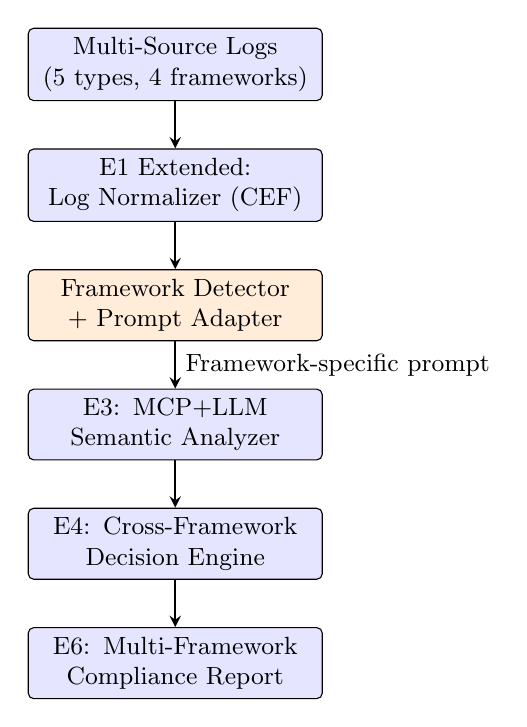
\begin{tikzpicture}[
    node distance=0.8cm,
    box/.style={rectangle, draw, fill=blue!10, text width=3.5cm, align=center, minimum height=0.8cm, font=\small, rounded corners=2pt},
    adapter/.style={rectangle, draw, fill=orange!15, text width=3.5cm, align=center, minimum height=0.8cm, font=\small, rounded corners=2pt},
    decision/.style={diamond, draw, fill=yellow!15, text width=2cm, align=center, font=\small},
    arrow/.style={->, >=stealth, thick}
]
\node[box] (input) {Multi-Source Logs\\(5 types, 4 frameworks)};
\node[box, below=0.6cm of input] (norm) {E1 Extended:\\Log Normalizer (CEF)};
\node[adapter, below=0.6cm of norm] (adapter) {Framework Detector\\+ Prompt Adapter};
\node[box, below=0.6cm of adapter] (e3) {E3: MCP+LLM\\Semantic Analyzer};
\node[box, below=0.6cm of e3] (e4) {E4: Cross-Framework\\Decision Engine};
\node[box, below=0.6cm of e4] (report) {E6: Multi-Framework\\Compliance Report};

\draw[arrow] (input) -- (norm);
\draw[arrow] (norm) -- (adapter);
\draw[arrow] (adapter) -- node[right, font=\small] {Framework-specific prompt} (e3);
\draw[arrow] (e3) -- (e4);
\draw[arrow] (e4) -- (report);
\end{tikzpicture}
\caption{Extended architecture supporting cross-domain log normalization and cross-framework prompt adaptation while preserving the validated Rwanda NCSA baseline}
\label{fig:arch_v2}
\end{figure}

\subsection*{B.\quad Cross-Framework Control Mapping Schema}

\begin{table}[h]
\centering
\caption{Cross-Framework Control Mapping (Sample)}
\label{tab:cross_framework}
\begin{tabular}{@{}p{2.5cm}p{2.5cm}p{2.5cm}p{2.5cm}p{2.5cm}@{}}
\toprule
\textbf{Control Class} & \textbf{Rwanda NCSA} & \textbf{Kenya CMCA} & \textbf{Nigeria NITDA} & \textbf{SA POPIA} \\
\midrule
Account Mgmt & AC-2 & Sec. 16 (Access) & NITDA-AC-1 & Sec. 22 (Authoriz.) \\
Failed Login & AC-7 & Sec. 19 (Auth.) & NITDA-AC-4 & --- \\
Audit Logging & AU-2 & Sec. 26 (Logs) & NITDA-AU-1 & Sec. 19 (Records) \\
Encryption at Rest & SC-28 & Sec. 31 (Encrypt.) & NITDA-SC-3 & Sec. 19 (Protect.) \\
Malware Protection & SI-3 & Sec. 24 (Malware) & NITDA-SI-2 & --- \\
Boundary Protection & SC-7 & Sec. 28 (Firewall) & NITDA-SC-1 & Sec. 21 (Access) \\
\bottomrule
\end{tabular}
\end{table}

\subsection*{C.\quad On-Premise LLM Evaluation Pipeline}

To address the cloud API dependency limitation, the extension evaluates three deployment tiers:

\begin{table}[h]
\centering
\caption{LLM Deployment Tier Comparison}
\label{tab:llm_tiers}
\begin{tabular}{@{}p{3cm}p{3cm}p{2cm}p{2cm}p{3cm}@{}}
\toprule
\textbf{Tier} & \textbf{Model} & \textbf{Size} & \textbf{Hardware} & \textbf{Cost Model} \\
\midrule
Cloud API (baseline) & Claude Sonnet / GPT-4 & API-based & No GPU & \$0.003--\$0.015/1K tokens \\
On-Premise Large & Llama-3.1-8B-Instruct & 8B params & CPU only & One-time download \\
On-Premise Small & Mistral-7B-Instruct-v0.3 & 7B params & CPU only & One-time download \\
Quantized (4-bit) & Llama-3.1-8B-Q4\_K\_M & $\sim$4.9GB & 8GB RAM & One-time download \\
\bottomrule
\end{tabular}
\end{table}

\bigskip

%==========================================================================
\section*{IV.\quad Updated Data Pipeline and Preprocessing Steps}

\begin{enumerate}
    \item \textbf{Ingestion:} Raw logs collected from 8 sources in their native formats (Syslog RFC 5424, EVTX XML, NetFlow v9, JSON, BGL format, HDFS format).

    \item \textbf{Normalization:} Each log is mapped to a canonical 8-field CEF schema: \texttt{timestamp}, \texttt{source\_host}, \texttt{event\_type}, \texttt{severity}, \texttt{user}, \texttt{resource}, \texttt{message}, \texttt{outcome}. Fields unavailable in a source format are populated as \texttt{NULL} with a source-specific flag.

    \item \textbf{Framework Detection:} A lightweight classifier (regex-based rule set) detects the applicable regulatory framework based on institution metadata (country code, sector tag) attached during ingestion.

    \item \textbf{Prompt Adaptation:} The Framework Detector selects one of four prompt templates (NCSA, CMCA, NITDA, POPIA) and injects the normalized log plus the relevant control family definitions into the LLM context window via MCP tool call.

    \item \textbf{Evidence Classification:} The MCP+LLM semantic analyzer returns: control IDs, compliance status (compliant / non-compliant / partial), confidence score, evidence indicators, and remediation notes---identical output schema to v1.0 for backward compatibility.

    \item \textbf{Cross-Framework Decision:} Engine 4 evaluates compliance decisions against both the primary framework (e.g., NCSA) and mapped equivalent controls in secondary frameworks, enabling multi-framework compliance gap analysis in a single audit run.

    \item \textbf{Evaluation Metrics:} Per-log-type and per-framework F1 scores, zero-shot vs. prompt-adapted accuracy, inference latency per deployment tier, and cost-per-1000-logs for each tier.
\end{enumerate}

\bigskip

%==========================================================================
\section*{V.\quad Dataset Description and Justification}

\begin{table}[h]
\centering
\caption{Dataset Justification per Source}
\label{tab:justification}
\begin{tabular}{@{}p{3cm}p{5cm}p{5cm}@{}}
\toprule
\textbf{Dataset} & \textbf{Justification} & \textbf{NCSA Relevance} \\
\midrule
SecRepo auth.log~[1] & Baseline from v1.0; provides zero-shot starting point for cross-log comparison & AC-7, IA-2, AU-2 \\
LogHub BGL~[2] & Production HPC system logs; tests semantic generalization beyond authentication events & AU-2, CM-6, SI-4 \\
LogHub HDFS~[2] & Distributed storage logs; evaluates SC-28 (protection at rest) and AU-9 (audit protection) & SC-28, AU-9 \\
EVTX-ATTACK-SAMPLES~[3] & Real Windows attack event logs; challenges SI-4 (system monitoring) and IA-5 (authenticator mgmt) & AC-2, IA-5, SI-4 \\
CICIDS 2017~[4] & Labeled network intrusion dataset covering 15 attack types; evaluates SC-7, SI-3 & SC-7, SI-3, SI-4 \\
Kenya / Nigeria / SA Synthetic & Fills regulatory gap for African frameworks not covered by public datasets; generated from published framework text & Multi-framework \\
\bottomrule
\end{tabular}
\end{table}

\bigskip

%==========================================================================
\section*{VI.\quad Expected Outcomes}

\subsection*{A.\quad Quantitative Deliverables}

\begin{enumerate}
    \item \textbf{Cross-Domain Accuracy Matrix:} Per-log-type F1 scores for both zero-shot and prompt-adapted MCP+LLM analysis (8 log sources $\times$ 4 frameworks = 32 evaluation cells).
    \item \textbf{Cross-Framework Transfer Table:} F1 score comparison when NCSA-trained prompts are applied to Kenya CMCA, Nigeria NITDA, and South Africa POPIA logs, and when framework-specific prompts are used.
    \item \textbf{Deployment Tier Comparison:} Latency, memory usage, cost-per-1000-logs, and accuracy for Cloud API vs. Llama-3.1-8B vs. Mistral-7B vs. 4-bit quantized variants.
    \item \textbf{Log Normalization Coverage Report:} Percentage of fields successfully normalized per source format, and impact of NULL fields on classification accuracy.
\end{enumerate}

\subsection*{B.\quad Qualitative Insights}

\begin{enumerate}
    \item Which control families are most sensitive to log type (authentication-centric vs. network-centric)?
    \item Which African regulatory framework has the highest semantic overlap with Rwanda NCSA, enabling lowest-cost cross-framework adaptation?
    \item At what log volume threshold does on-premise quantized LLM deployment become more cost-effective than cloud API?
    \item Which log normalization gaps (NULL fields) most critically impact MCP+LLM compliance accuracy?
\end{enumerate}

\bigskip

%==========================================================================
\textbf{REFERENCES}

\begin{enumerate}[leftmargin=*, label={[\arabic*]}]

\item SecRepo, ``Security Data Samples Repository,'' 2024. [Online]. Available: https://www.secrepo.com/

\item S. He et al., ``Loghub: A Large Collection of System Log Datasets for AI-Driven Log Analytics,'' in \textit{Proc. IEEE ISSRE}, 2023. arXiv:2008.06448.

\item EVTX-ATTACK-SAMPLES, ``Real Windows Event Log Attack Samples,'' GitHub, 2024. [Online]. Available: https://github.com/sbousseaden/EVTX-ATTACK-SAMPLES

\item I. D. Sharafaldin, A. H. Lashkari, and A. A. Ghorbani, ``Toward Generating a New Intrusion Detection Dataset and Intrusion Traffic Characterization,'' in \textit{Proc. ICISSP}, 2018.

\item Rwanda National Cyber Security Authority (NCSA), ``Minimum Cybersecurity Standards,'' 2023.

\item Republic of Kenya, ``Computer Misuse and Cybercrimes Act,'' 2018, amended 2024. [Online]. Available: https://kenyalaw.org

\item Federal Republic of Nigeria, ``National Information Technology Development Agency (NITDA) Cybersecurity Framework,'' 2024.

\item Republic of South Africa, ``Protection of Personal Information Act (POPIA), Act No. 4 of 2013,'' Government Gazette, 2020.

\item M. A. Ferrag et al., ``Evaluating Large Language Models Effectiveness for Flow-Based Intrusion Detection,'' \textit{Artificial Intelligence Review}, Springer, 2025. doi: 10.1007/s10462-025-11432-2.

\item N. Ahmad et al., ``Lightweight Quantized XGBoost for Botnet Detection in Resource-Constrained IoT Networks,'' \textit{IoT}, MDPI, vol. 6, no. 4, 2025. doi: 10.3390/iot6040070.

\item Anthropic, ``Introducing the Model Context Protocol,'' \textit{Anthropic Blog}, Nov. 2024. [Online]. Available: https://www.anthropic.com/news/model-context-protocol

\item C. Wang et al., ``Model Context Protocol (MCP): Landscape, Security Threats, and Future Research Directions,'' \textit{arXiv:2503.23278}, 2025.

\end{enumerate}

\end{document}
